\documentclass[mathserif,16pt,xcolor=table]{beamer}

% Load Beamer Style Theme
% TAMU Based
\usepackage{tamu_beamer}
% \usepackage[skip=0pt]{caption}

% Specifiy the location of images to be used
\graphicspath{{figures/}}

% ------------------------------------------------------------
% ------------------------------------------------------------
% ------------------------------------------------------------
% ----------------TITLE PAGE----------------------------------
% ------------------------------------------------------------
% ------------------------------------------------------------
% ------------------------------------------------------------
% Document Title Page
\title{Surface wave supporting structures in the terahertz and optical frequency domains}
% \subtitle{Preliminary Exam}
\author[Hasan Tahir Abbas]{Hasan Tahir Abbas\\~\\{\small {Supervised by: Dr. Robert D. Nevels}}}
\institute{Department of Electrical  \& Computer Engineering\\ \mbox{} \\ \pgfuseimage{tamuecenbig}}
\date[Summer 2017]{\today}
% ------------------------------------------------------------
% ------------------------------------------------------------
% ------------------------------------------------------------
% ------------------------------------------------------------
% ------------------------------------------------------------
% ------------------------------------------------------------
% ------------------------------------------------------------
% ------------------------------------------------------------
% ------------------------------------------------------------
% ------------------------------------------------------------
% ------------------------------------------------------------
% ------------------------------------------------------------
% ------------------------------------------------------------
% ------------------------------------------------------------
\begin{document}

% Reduce space around equations and subequations
\preto\subequations{\ifhmode\unskip\fi}
\AtBeginEnvironment{subequations}{\ifhmode\unskip\fi}
\AtBeginEnvironment{equation}{\ifhmode\unskip\fi}

% Draw Boxes in the footer with pertinent info
\tikzstyle{block} = [rectangle, draw, rounded corners, shade, top color=white, text width=5em,
bottom color=blue!50!black!20, draw=blue!40!black!60, very thick, text centered, minimum height=4em]
\tikzstyle{line} = [draw, -latex']
\tikzstyle{cloud} = [draw, ellipse,top color=white, bottom color=red!20, node distance=2cm, minimum height=2em]

% Tick Style
\beamertemplateballitem
% \beamertemplatetransparentcoveredhigh

\frame{\titlepage}


% Add TAMU logo on each slide in the north-east side
% Shifted to be right at the edge
%
% NOTE: Will have to compile twice
%
\addtobeamertemplate{frametitle}{}{%
\begin{tikzpicture}[remember picture,overlay]
  \node[anchor=north east,yshift=7pt,xshift=2pt] at (current page.north east) {
\includegraphics[height=.7cm]{ecen}};
\end{tikzpicture}}
% ------------------------------------------------------------
% ------------------------------------------------------------
% ------------------------------------------------------------
% ------------------------------------------------------------
% ------------------------------------------------------------
% ------------------------------------------------------------
% ------------------------------------------------------------
% ------------------------------------------------------------
% ------------------------------------------------------------
% ------------------------------------------------------------
% ------------------------------------------------------------
% ------------------------------------------------------------
% ------------------------------------------------------------
% ------------------------------------------------------------
\section{Outline}
\begin{frame}
  \frametitle{Outline}
  \begin{outline}[itemize]
    \1 Overview
    \1 Background
    \1 Theory and Methods
      \2 Subwavelength phenomena - Dispersion relations
      \2 Existence of plasmonic behavior - Sommerfeld Integral analysis
      \2 Surface Integral equation scheme
    \1 Applications
      \2 Super-resolution Imaging scheme
    \1 Conclusions
  \end{outline}
\end{frame}
% ------------------------------------------------------------
% ------------------------------------------------------------
% ------------------------------------------------------------
% ------------------------------------------------------------
% ------------------------------------------------------------
% ------------------------------------------------------------
% ------------------------------------------------------------
% ------------------------------------------------------------
% ------------------------------------------------------------
% ------------------------------------------------------------
% ------------------------------------------------------------
% ------------------------------------------------------------
% ------------------------------------------------------------
\section{Overview}
% ------------------------------------------------------------
% ------------------------------------------------------------
\begin{frame}
  \frametitle{Overview}
  % ----------------------------------------------------------
  % Talk about the significance of this research
  \begin{columns} % align columns
    \begin{column}{.5\textwidth} \vspace*{-1cm}
      \begin{outline}[itemize]
        \1 Plasmonics: subwavelength localization of electromagnetic (EM) fields
        \1 Bridging the THz gap
      \end{outline}
    \end{column}
    \begin{column}{.5\textwidth}
      % Use this to preserve fonts from Inkspace
      \begin{figure}
        \centering \hspace*{-0.75cm}
        \fontsize{6}{7}\selectfont
        \def\svgwidth{1.1\linewidth}
        \input{figures/scale.pdf_tex}
        \label{fig:spp_2deg}
        \caption{Communication Technologies at various frequencies}
      \end{figure}
      \end{column}%
    \end{columns}
  \end{frame}
  % ------------------------------------------------------------
  % ------------------------------------------------------------
  % ------------------------------------------------------------
  % ------------------------------------------------------------
  % ------------------------------------------------------------
  % ------------------------------------------------------------
  % ------------------------------------------------------------
  % ------------------------------------------------------------
  % ------------------------------------------------------------
  \begin{frame}
    \frametitle{Overview}
    \framesubtitle{Terahertz 2DES}
    % ----------------------------------------------------------
    % Talk about the significance of this research
    \begin{outline}[itemize]
      \1 Graphene
      \2 Grown separately, transfered to substrate
      \2 Currently not integrable to current electronics technology
      \2 Superior electronic properties
      \1 Semiconductor heterostructures
      \2 Conventional epitaxial semiconductor device fabrication techniques
      \2 On-chip integration with silicon electronics
    \end{outline}
  \end{frame}

  % ------------------------------------------------------------
  % ------------------------------------------------------------
  % ------------------------------------------------------------
  % ------------------------------------------------------------
  % ------------------------------------------------------------
  % ------------------------------------------------------------
  % ------------------------------------------------------------

  % ------------------------------------------------------------
  % ------------------------------------------------------------
  % ------------------------------------------------------------
  % ------------------------------------------------------------
  % ------------------------------------------------------------
  % ------------------------------------------------------------
  % ------------------------------------------------------------
  \section{Background}
  % ------------------------------------------------------------
  % ------------------------------------------------------------
  % ------------------------------------------------------------
  % ------------------------------------------------------------
  % ------------------------------------------------------------
  % ------------------------------------------------------------
  % ------------------------------------------------------------
  % ------------------------------------------------------------
  % ------------------------------------------------------------
  % ------------------------------------------------------------
  % ------------------------------------------------------------
  % ------------------------------------------------------------
  % ------------------------------------------------------------
  \begin{frame}
    \frametitle{Background}
    \framesubtitle{Plasmonics Overview}
    % ----------------------------------------------------------
    \begin{columns} % align columns
      \begin{column}{.5\textwidth}
        \begin{outline}[itemize]
          \1 Interfacial wave phenomena
            \2 Metal-dielectric interface
            \2 Semiconductor heterostructure
          \1 Surface plasmon polaritons (SPPs)
        \end{outline}
        %
        \begin{outline}[itemize]
          \1 Plasma frequency
          \2 Metals - Optical frequency
          \2 Semiconductors - Terahertz
        \end{outline}
        %
      \end{column}
      \begin{column}{.5\textwidth}
        % Use this to preserve fonts from Inkspace
        \begin{figure}
          \centering
          \fontsize{6}{7}\selectfont% Reduce the fontsize
          \def\svgwidth{.8\linewidth}
          \input{figures/spp.pdf_tex}
          \label{fig:spp}
          \caption{SPPs at optical frequencies}
        \end{figure}
        %
        \begin{figure}
          \centering
          \fontsize{6}{7}\selectfont
          \def\svgwidth{.8\linewidth}
          \input{figures/spp_2deg.pdf_tex}
          \label{fig:spp_2deg}
          \caption{SPPs in the THz regime}
        \end{figure}
        \end{column}%
      \end{columns}
    \end{frame}
    % ------------------------------------------------------------
    % ------------------------------------------------------------
    % ------------------------------------------------------------
    % ------------------------------------------------------------
    % ------------------------------------------------------------
    % ------------------------------------------------------------
    % ------------------------------------------------------------
    \begin{frame}
      \frametitle{Background}
      \framesubtitle{Surface Plasmon Polaritons}

      \begin{columns} % align columns
        \begin{column}{.5\textwidth}
          \begin{minipage}[T][.1\textheight][c]{\linewidth}
            \begin{outline}[itemize]
              \1 Slow surface waves
              \1 Reduced Wavelength
              \1 Focusing beyond the diffraction limit
            \end{outline}
            \begin{outline}[itemize]
              \1 Optical SPP
            \end{outline}
            \setlength{\belowdisplayshortskip}{-7pt}
            \setlength{\abovedisplayshortskip}{2pt}
            \begin{equation} \nonumber
              \Re \left[ \E_{\text{metal}}(\O)\right] < 0
            \end{equation}
            \begin{outline}[itemize]
              \1 THz SPP
            \end{outline}
            \begin{equation} \nonumber
              \Im \left[ \sigma_{s}(\O)\right] < 0
            \end{equation}
          \end{minipage}
        \end{column}
        \begin{column}{.5\textwidth}
          % Use this to preserve fonts from Inkspace
          \begin{figure}
            \centering \hspace*{-1.25cm}
            \fontsize{6}{7}\selectfont
            \def\svgwidth{1.1\linewidth}
            \input{figures/spps_comp.pdf_tex}
            \label{fig:spp_2deg}
            \caption{Dispersion Curve comparison}
          \end{figure}
          \end{column}%
        \end{columns}
      \end{frame}
      % ------------------------------------------------------------
      % ------------------------------------------------------------
      % ------------------------------------------------------------
      % ------------------------------------------------------------
      % ------------------------------------------------------------
      % ------------------------------------------------------------
      % ------------------------------------------------------------
      % ------------------------------------------------------------
      \begin{frame}
        \frametitle{Background}
        \framesubtitle{Optical Nanoantennas}

        \begin{columns} % align columns
          \begin{column}{.45\textwidth}
            % \begin{minipage}[T][.1\textheight][c]{\linewidth}
            \vspace*{-1cm}
              \begin{outline}[itemize]
                \1 Convert Localized near-field to efficient far-field radiation
                \1 Low Q-factor
                \1 Extremely small size
                \1 \color{red}{High Purcell Factor}
              \end{outline}
              % \setlength{\belowdisplayshortskip}{-7pt}
              % \setlength{\abovedisplayshortskip}{2pt}
            \begin{equation} \nonumber
              {P}  = \frac{{Q}}{{V}}
            \end{equation}
            \begin{outline}[itemize]
              \1 Directive radiation
            \end{outline}
            % \end{minipage}
            %
          \end{column}
          %
          \begin{column}{.55\textwidth}
            \vspace*{-1cm}
            % Use this to preserve fonts from Inkspace
            \begin{figure}
              \centering \hspace*{-1.25cm}
              \fontsize{6}{7}\selectfont
              \def\svgwidth{1.1\linewidth}
              \input{figures/curto.pdf_tex}
              \caption{Optical resonant cavities for electric field enhancement}
            \end{figure}
            \end{column}%
          \end{columns}
        \end{frame}
      %   % ------------------------------------------------------------
      %   % ------------------------------------------------------------
      %   % ------------------------------------------------------------
      %   % ------------------------------------------------------------
      %   % ------------------------------------------------------------
      %   % ------------------------------------------------------------
      %   % ------------------------------------------------------------
      %   % ------------------------------------------------------------
        \begin{frame}
          \frametitle{Background}
          \framesubtitle{Optical Nanoantennas (contd.)}

          \begin{columns} % align columns
            \begin{column}{.45\textwidth}
              \begin{minipage}[T][.1\textheight][c]{\linewidth}
                \begin{outline}[itemize]
                  \1 Scaled-down microwave antenna designs
                  \1 Shift of resonance with width unlike in microwave regime
                \end{outline}
                \begin{figure}
                  \includegraphics[scale=.03]{bowtie_field_map.png}
                  % \caption{Subwavelength Transmission through a Silver slit}
                \end{figure}
              \end{minipage}
            \end{column}
            %
            \begin{column}{.55\textwidth}
              % Use this to preserve fonts from Inkspace
              \vspace{-1.75cm}
              \begin{figure}
                \centering
                \subfloat{\includegraphics[height = 1.4in]{generate_fig8c.tikz}
                \label{fig:sim_his}}

                \centering \vspace{-.25cm}
                \subfloat{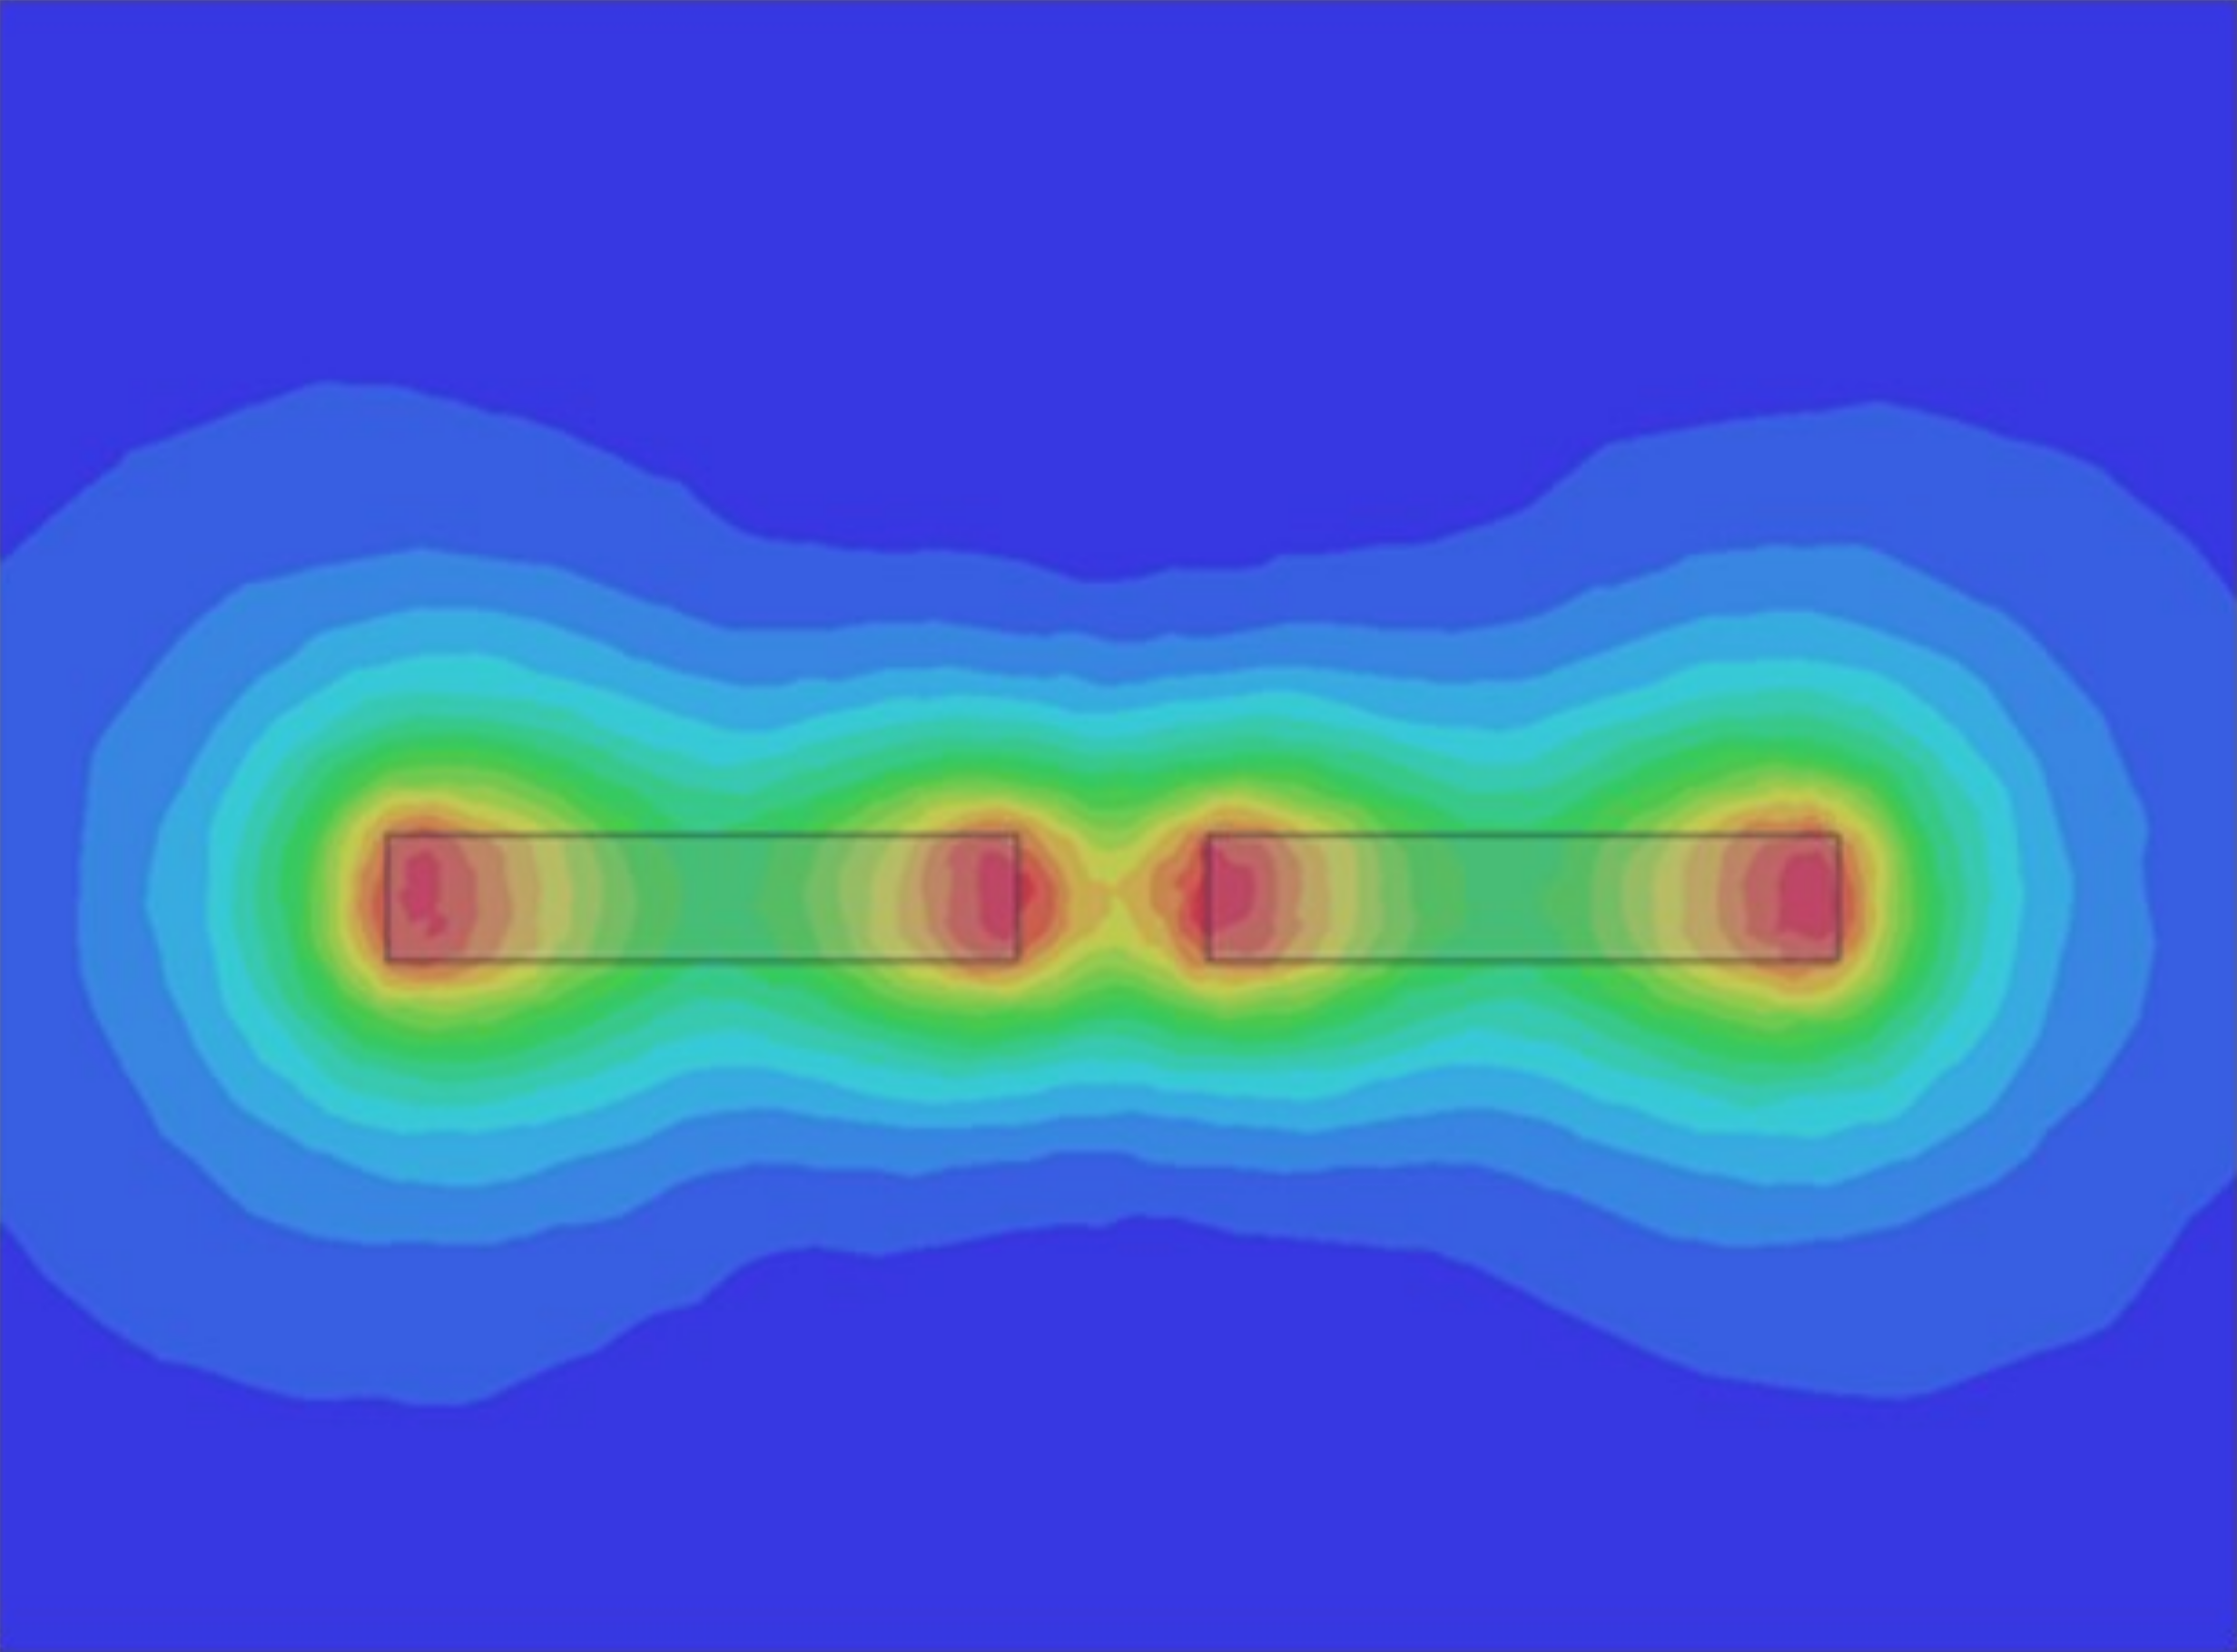
\includegraphics[height = .8in]{fig8_a.png}
                \label{fig:narrow}}

                \centering \vspace{-.25cm}
                \subfloat{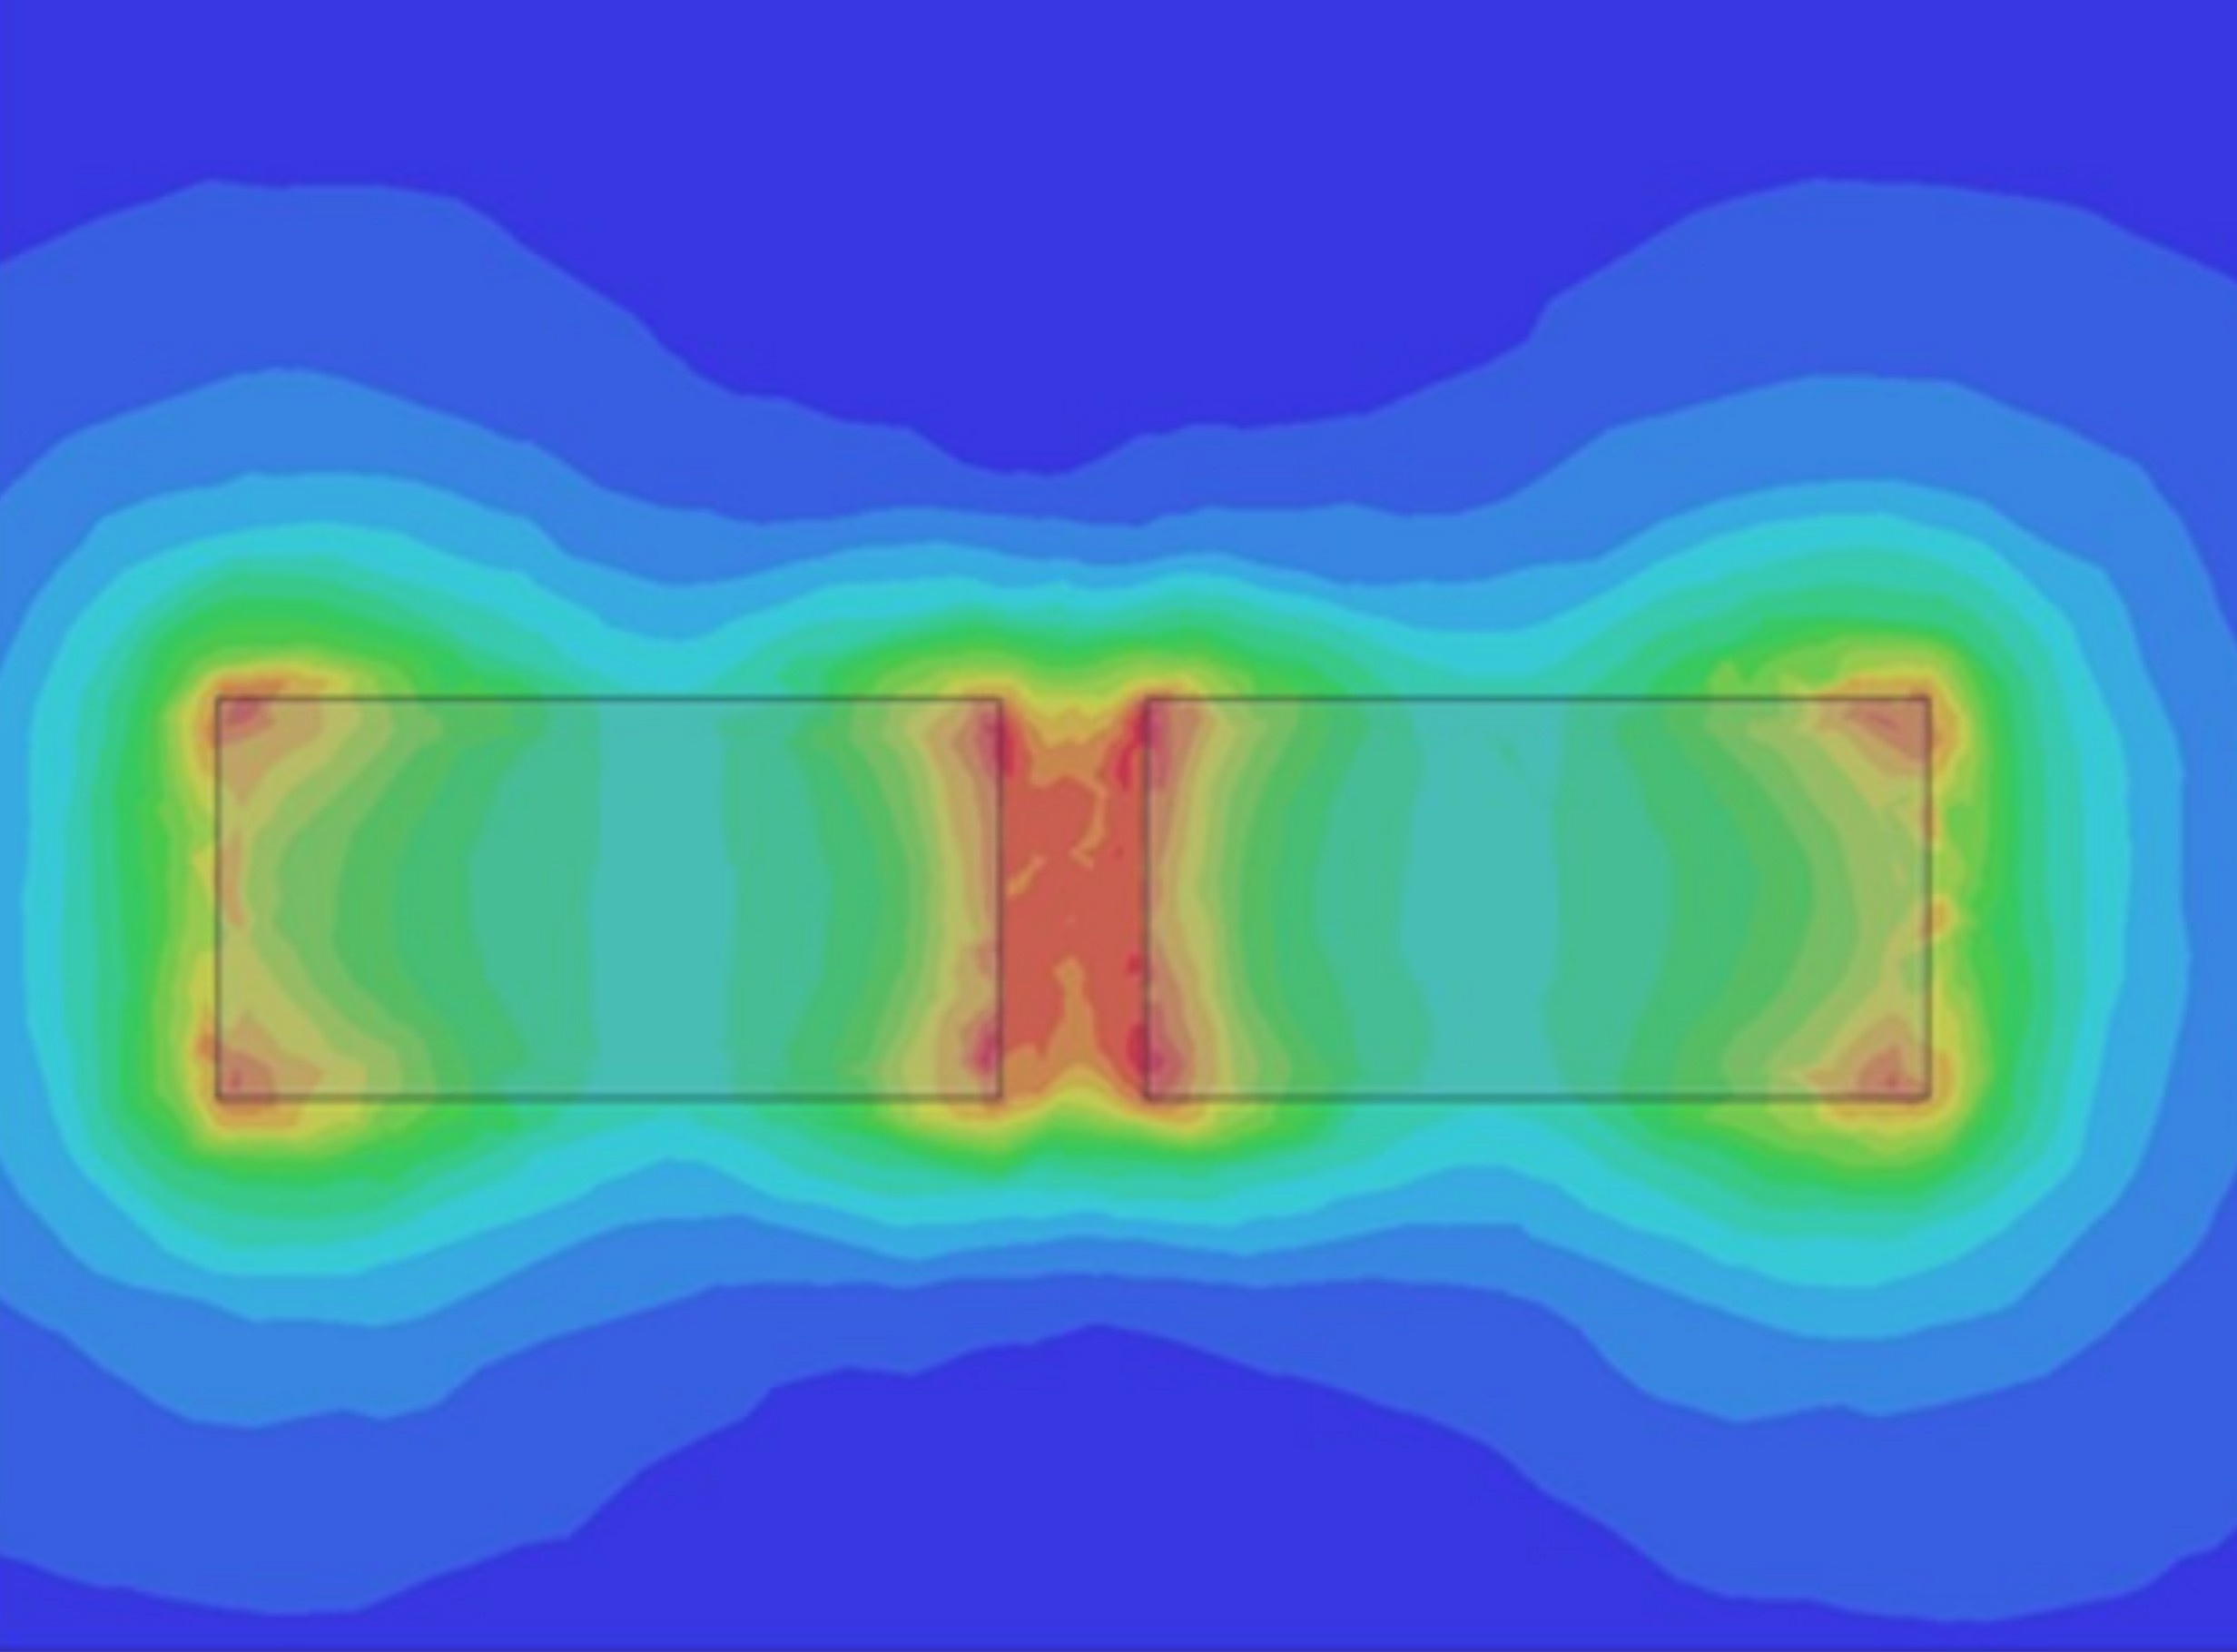
\includegraphics[height = .8in]{fig8_d.png}
                \label{fig:wide}}
                % \caption{(a) Maximum enhancement of a gold nanodipole excited at \SI{550}{\nm} (b) narrow and (c) wide profile. A narrow structure does not maintain resonance when widened without also changing its length.}
                \label{fig:simulationop}
              \end{figure}
              % \vspace*{-1.5cm}
              % \begin{figure}
              %   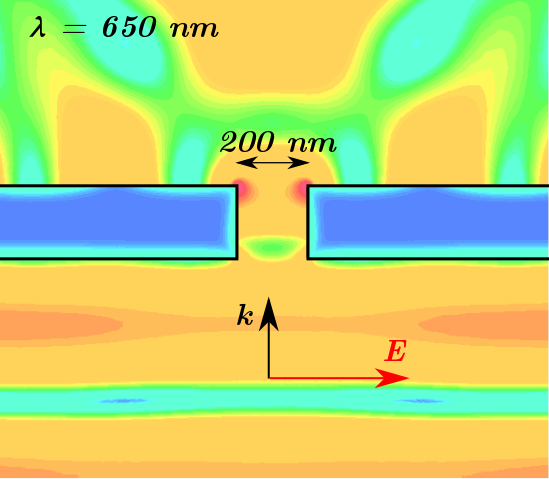
\includegraphics[scale=.2]{E_squared_final.png}
              % \end{figure}
              % \vspace*{-1cm}
              % \begin{figure} \hspace*{-.25cm} \centering
              %   \includegraphics[width = 1.05\linewidth]{fig13.jpg}
              %   \label{fig:cst_simulation}
              % \end{figure}
              \end{column}%
            \end{columns}
          \end{frame}
      %     % ------------------------------------------------------------
      %     % ------------------------------------------------------------
      %     % ------------------------------------------------------------
      %     % ------------------------------------------------------------
      %     % ------------------------------------------------------------
      %     % ------------------------------------------------------------
      %     % ------------------------------------------------------------
      %     % ------------------------------------------------------------
          \begin{frame}
            \frametitle{Background}
            \framesubtitle{Two-dimensional Electron Gas (2DEG)}

            \begin{columns} % align columns
              \begin{column}{.5\textwidth}
                \begin{minipage}[T][.1\textheight][c]{\linewidth}
                  \begin{outline}[itemize]
                    \1 Semiconductor Heterostructure in high electron mobility transistor (HEMT)
                    \1 High concentration of free electrons ($\sim \num{1e11}-\SI{1e14}{\cm^{-2}}$)
                    \1 Very high Mobility ($\sim \num{1e3}-\SI{1e6}{\cm^{2}/V/s}$)
                    \1 Formation of Quantum Well
                      \2 Two-dimensional confinement of electrons
                  \end{outline}
                \end{minipage}
                %
              \end{column}
              %
              \begin{column}{.5\textwidth}
                % Use this to preserve fonts from Inkspace
                \begin{figure}
                  \centering
                  \fontsize{6}{7}\selectfont
                  \def\svgwidth{.8\linewidth}
                  \input{figures/hemt2.pdf_tex}
                  \caption{Typical GaAs/AlGaAs HEMT}
                \end{figure}
                \begin{figure}
                  \centering \vspace*{-1cm}
                  \fontsize{6}{7}\selectfont
                  \def\svgwidth{.8\linewidth}
                  \input{figures/2deg_bandgap.pdf_tex}
                  \caption{Band diagram of a GaAs/AlGaAs heterostructure}
                \end{figure}
                \end{column}%
              \end{columns}
            \end{frame}
      %       % ------------------------------------------------------------
      %       % ------------------------------------------------------------
      %       % ------------------------------------------------------------
      %       % ------------------------------------------------------------
      %       % ------------------------------------------------------------
      %       % ------------------------------------------------------------
      %       % ------------------------------------------------------------
      %       % ------------------------------------------------------------
            \begin{frame}
              \frametitle{Background}
              \framesubtitle{2DEG (contd.)}

              \begin{columns} % align columns
                \begin{column}{.5\textwidth}
                  \begin{minipage}[T][.1\textheight][c]{\linewidth}
                    \begin{outline}[itemize]
                      \1 Plasma waves in 2DEG
                      \1 Dyakonov-Shur instability
                        \2 Voltage bias at source and drain terminals
                        \2 Plasma resonance
                        \2 THz emission
                      \1 Electronic Flute
                        \2 Tunable resonance with gate voltage
                    \end{outline}
                  \end{minipage}
                  %
                \end{column}
                %
                \begin{column}{.5\textwidth}
                  % Use this to preserve fonts from Inkspace
                  \begin{figure}
                    \hspace*{-.55cm}
                    \fontsize{6}{7}\selectfont
                    \def\svgwidth{1.1\linewidth}
                    \input{figures/flute_2deg2.pdf_tex}
                    % \caption{Typical GaAs/AlGaAs HEMT}
                  \end{figure}
                  \begin{equation} \nonumber
                    \begin{split}
                      \lambda &= \frac{c}{f} \\
                      & \Longrightarrow  300 \u \mathrm{m}
                    \end{split}
                    \label{eq:disp_TE_two}
                  \end{equation}
                  \end{column}%
                \end{columns}
              \end{frame}
      %         % ------------------------------------------------------------
      %         % ------------------------------------------------------------
      %         % ------------------------------------------------------------
      %         % ------------------------------------------------------------
      %         % ------------------------------------------------------------
      %         % ------------------------------------------------------------
      %         % -------------------THEORY-----------------------------------
      %         % ------------------------------------------------------------
      %         % ------------------------------------------------------------
      %         % ------------------------------------------------------------
      %         % ------------------------------------------------------------
      %         % ------------------------------------------------------------
      %         % ------------------------------------------------------------
      %         % ------------------------------------------------------------
      %         % ------------------------------------------------------------
      %         % ------------------------------------------------------------
      %         % Beginning of the actual content
      \section{Theory and Methods}
      \begin{frame}
        \frametitle{Theory}
        \framesubtitle{SPP Dispersion Relation}
        \begin{columns}[T] % align columns
          \begin{column}{.5\textwidth}
            \begin{outline}[itemize]
              \1 SPP pole
            \end{outline}
            \begin{equation} \nonumber
              k_{sp}=\frac{\O}{c}\sqrt {\dfrac {\E_{1}\E_{2}(\O)} {\E_{1} + \E_{2}(\O)}}
              \label{eq:dis_spp}
            \end{equation}
            \begin{outline}[itemize]
              \1 Accurate material description
            \end{outline}
            \begin{equation} \nonumber
              \E_2(\O) = \E_{\inf} - \frac{\O_{d}^{2}}{\O^2 - \j\gamma \O} + \sum \limits_{i = 1}^N G_i(\O)
              \label{eq:eps_drude_cp}
            \end{equation}
            \begin{equation} \nonumber
              G_i(\O) = C_i \left[ \frac{e^{\j \phi_i}}{\O_i + \O - \j \Gamma_i} + \frac{e^{-\j \phi_i}}{\O_i - \O + \j \Gamma_i} \right]
              \label{eq:CP_terms}
            \end{equation}
          \end{column}
          \begin{column}[T]{.45\textwidth}
            \vspace*{-2cm}
            \centering
            \begin{figure}
              \subfloat{\includegraphics[height = 1.5in]{ep_silver.tikz}
              \label{fig:ep_gold}}

              \subfloat{\hspace*{-.1cm} \includegraphics[height = 1.5in]{disp_silver.tikz}
              \label{fig:ep_silver}}
            \end{figure}
          \end{column}
        \end{columns}
      \end{frame}
      %     % ------------------------------------------------------------
      %     % ------------------------------------------------------------
      %     % ------------------------------------------------------------
      %     % ------------------------------------------------------------
      %     % ------------------------------------------------------------
      %     % ------------------------------------------------------------
      %     % ------------------------------------------------------------
      \begin{frame}
        \frametitle{Theory and Methods}
        \framesubtitle{2DEG Circuit model}
        \begin{columns} % align columns
          \begin{column}{.5\textwidth}
            \begin{minipage}[T][.1\textheight][c]{\linewidth}
              \begin{outline}[itemize]
                \1 Drude-Lorentz Surface Conductivity
              \end{outline}
              %
              \begin{equation} \nonumber
                \sigma_s = \frac{N_s e^2}{m^{\ast}}\frac{\tau}{1 + \j \tau \O}
                \label{eq:Y2deg}
              \end{equation}
              \begin{itemize}
                \item[] {\makebox[.3cm][l]{$N_s$} - Surface charge density}
                \item[] {\makebox[.3cm][l]{$\tau$} - Scattering time}
                \item[] {\makebox[.3cm][l]{$m^{\ast}$} - Effective electron mass}
              \end{itemize}
              \begin{outline}[itemize]
                \1 Equivalent Circuit
                \end{outline}
                \begin{equation} \nonumber
                  \sigma_s = \frac{1}{Z} = \frac{1}{R + {1}/{\j \O C}}
                  \label{eq:simga_TL}
                \end{equation}
            \end{minipage}
          \end{column}
          %
          \begin{column}{.5\textwidth}
            % Use this to preserve fonts from Inkspace
            \begin{figure} \vspace*{-1.75cm}
              \includegraphics[height = 2.0in]{cond_2deg_gan.tikz}
              \label{fig:cond_2deg}
              \caption{Room temperature GaN/AlGaN 2DEG surface conductivity}
            \end{figure}
            %
            \begin{figure} \vspace*{-.75cm}
              \centering
              \fontsize{6}{7}\selectfont
              \def\svgwidth{.75\linewidth}
              \input{figures/circuit.pdf_tex}
              % \caption{Typical GaAs/AlGaAs HEMT}
            \end{figure}
            \end{column}%
          \end{columns}
        \end{frame}
      %           % ------------------------------------------------------------
      %           % ------------------------------------------------------------
      %           % ------------------------------------------------------------
      %           % ------------------------------------------------------------
      %           % ------------------------------------------------------------
      %           % ------------------------------------------------------------
      %           % ------------------------------------------------------------
      \begin{frame}
        \frametitle{Theory and Methods}
        \framesubtitle{Dispersion Relation for a 2D Sheet}
        \begin{columns}[T] % align columns
          \begin{column}{.5\textwidth}
            \begin{outline}[itemize]
              \1 Conductive Sheet in freespace
              \1 TM mode surface wave
            \end{outline}
            \begin{equation} \nonumber
              k^{\mathrm{TM}}_{\mathrm P} = \frac{\O}{c} \sqrt{1 - \left(\frac{2}{\eta_0 \sigma_s}\right)^2}
              \label{eq:TM_pole}%
            \end{equation}
            \begin{outline}[itemize]
              \1 Below plasma frequency
              \end{outline}
            \begin{equation} \nonumber
              \Im \sigma_s < 0
              \label{eq:2deg_surface_wave}%
            \end{equation}%
            \begin{outline}[itemize]
              \1 At low temperature
              \end{outline}%
            \begin{equation} \nonumber
              \Im |\sigma_s| \gg \Re |\sigma_s|
              \label{eq:2deg_low_loss}
            \end{equation}
          \end{column}
          \begin{column}[T]{.45\textwidth}
            \vspace*{-2cm}
            \centering
            \begin{figure}
              \subfloat{\includegraphics[height = 1.5in]{disp_gaas_sheet_77.tikz}
              \label{fig:disp_2deg_77}}

              \subfloat{\hspace*{-.1cm} \includegraphics[height = 1.5in]{disp_gaas_sheet_rt.tikz}
              \label{fig:disp_2deg_rt}}
            \end{figure}
          \end{column}
        \end{columns}
      \end{frame}
      %           % ------------------------------------------------------------
      %           % ------------------------------------------------------------
      %           % ------------------------------------------------------------
      %           % ------------------------------------------------------------
      %           % ------------------------------------------------------------
      %           % ------------------------------------------------------------
      %           % ------------------------------------------------------------
      \begin{frame}
        \frametitle{Theory and Methods}
        \framesubtitle{Dispersion Relation - Multilayer structures}
        \begin{columns}[T] % align columns
          \begin{column}{.45\textwidth}
            \begin{outline}[itemize]
              \1 Equivalent transmission line (TL) network
              \1 Dispersion relation
                \2 Transverse resonance condition
            \end{outline}
            \begin{equation} \nonumber
              Y^{\uparrow}(z_0) + Y^{\downarrow}(z_0) + Y_{\sigma} = 0.
              \label{eq:dispersion}
            \end{equation}
            \begin{outline}[itemize]
              \1 Different configurations
                \2 Gated
                \2 Ungated
                \2 Backgated
              \end{outline}
          \end{column}
          \begin{column}[T]{.65\textwidth}
            \vspace*{-1cm} \hspace*{-2cm}
            \begin{figure}
              \centering \hspace*{-.5cm}
              \fontsize{6}{7}\selectfont
              \def\svgwidth{1.2\linewidth}
              \input{figures/mlayers.pdf_tex}
              % \caption{Typical GaAs/AlGaAs HEMT}
            \end{figure}
          \end{column}
        \end{columns}
      \end{frame}
      %           % ------------------------------------------------------------
      %           % ------------------------------------------------------------
      %           % ------------------------------------------------------------
      %           % ------------------------------------------------------------
      %           % ------------------------------------------------------------
      %           % ------------------------------------------------------------
      %           % ------------------------------------------------------------
      \begin{frame}
        \frametitle{Theory and Methods}
        \framesubtitle{Dispersion Relation - Ungated 2DEG}
        \begin{columns}[T] % align columns
          \begin{column}{.5\textwidth}
            \begin{equation} \nonumber
              Y^{\uparrow} = Y_{2} \frac{1 - \Gamma^{\uparrow}}{1 + \Gamma^{\uparrow}}
            \end{equation}

            \begin{equation} \nonumber
              \Gamma^{\uparrow} = \frac{Y_2 - Y_1}{Y_2 + Y_1} \e^{-2\j k_{z2}\, h}
            \end{equation}

            \begin{equation} \nonumber
              Y^{\downarrow} = Y_{3}
            \end{equation}
            \begin{itemize}
              \item[] GaN/AlGaN heterostructure
              \item[] {\makebox[.3cm][l]{$N_s$} - \SI{5e13}{\cm^{-2}}}
              \item[] {\makebox[.3cm][l]{$\tau$} - \SI{1.4e-10}{\s}}
              \item[] {\makebox[.3cm][l]{$m^{\ast}$} - $0.2 m_e$}
              \item[] {\makebox[.3cm][l]{$ h$} - \SI{20}{\nm}}
            \end{itemize}
          \end{column}
          \begin{column}[T]{.45\textwidth}
            \vspace*{-1cm}
            \begin{figure}
              \centering
              \fontsize{6}{7}\selectfont
              \def\svgwidth{1.\linewidth}
              \input{figures/ungated.pdf_tex}
              % \caption{Typical GaAs/AlGaAs HEMT}
            \end{figure}
            \begin{figure} \vspace*{-.5cm} \centering
              \includegraphics[height = 1.5in]{ungated_disp.tikz}
              \label{fig:cond_2deg}
            \end{figure}
          \end{column}
        \end{columns}
      \end{frame}
      %           % ------------------------------------------------------------
      %           % ------------------------------------------------------------
      %           % ------------------------------------------------------------
      %           % ------------------------------------------------------------
      %           % ------------------------------------------------------------
      %           % ------------------------------------------------------------
      %           % ------------------------------------------------------------
      \begin{frame}
        \frametitle{Theory and Methods}
        \framesubtitle{Dispersion Relation - Gated 2DEG}
        \begin{columns}[T] % align columns
          \begin{column}{.5\textwidth}
            \begin{equation} \nonumber
              Y^{\uparrow} = - Y_{2} \coth (k_{z2} h)
            \end{equation}
            \begin{equation} \nonumber
              Y^{\downarrow} = Y_{3}
            \end{equation}
            \begin{itemize}
              \item[] GaN/AlGaN heterostructure
              \item[] {\makebox[.3cm][l]{$N_s$} - \SI{5e13}{\cm^{-2}}}
              \item[] {\makebox[.3cm][l]{$\tau$} - \SI{1.4e-10}{\s}}
              \item[] {\makebox[.3cm][l]{$m^{\ast}$} - $0.2 m_e$}
              \item[] {\makebox[.3cm][l]{$ h$} - \SI{20}{\nm}}
            \end{itemize}
          \end{column}
          \begin{column}[T]{.45\textwidth}
            \vspace*{-1cm}
            \begin{figure}
              \centering
              \fontsize{6}{7}\selectfont
              \def\svgwidth{1.\linewidth}
              \input{figures/gated.pdf_tex}
              % \caption{Typical GaAs/AlGaAs HEMT}
            \end{figure}
            \begin{figure} \vspace*{-.5cm} \centering
              \includegraphics[height = 1.5in]{backgated_disp.tikz}
              \label{fig:cond_2deg}
            \end{figure}
          \end{column}
        \end{columns}
      \end{frame}
      %           % ------------------------------------------------------------
      %           % ------------------------------------------------------------
      %           % ------------------------------------------------------------
      %           % ------------------------------------------------------------
      %           % ------------------------------------------------------------
      %           % ------------------------------------------------------------
      %           % ------------------------------------------------------------
      \begin{frame}
        \frametitle{Theory and Methods}
        \framesubtitle{Dispersion Relation - Backgated 2DEG}
        \begin{columns}[T] % align columns
          \begin{column}{.5\textwidth}
            \begin{equation} \nonumber
              Y^{\uparrow} = Y_{2} \frac{1 - \Gamma^{\uparrow}}{1 + \Gamma^{\uparrow}}
            \end{equation}
            \begin{equation} \nonumber
              \Gamma^{\uparrow} = \frac{Y_2 - Y_1}{Y_2 + Y_1} \e^{-2\j k_{z2}\, h}
            \end{equation}
            \begin{equation} \nonumber
              Y^{\downarrow} = - Y_{3} \coth (k_{z3} d)
            \end{equation}
            \begin{itemize}
              \item[] GaN/AlGaN heterostructure
              \item[] {\makebox[.3cm][l]{$N_s$} - \SI{5e13}{\cm^{-2}}}
              \item[] {\makebox[.3cm][l]{$\tau$} - \SI{1.4e-10}{\s}}
              \item[] {\makebox[.3cm][l]{$m^{\ast}$} - $0.2 m_e$}
              \item[] {\makebox[.3cm][l]{$ h$} - \SI{20}{\nm}}
              \item[] {\makebox[.3cm][l]{$ d$} - \SI{50}{\nm}}
            \end{itemize}
          \end{column}
          \begin{column}[T]{.45\textwidth}
            \vspace*{-1cm}
            \begin{figure}
              \centering
              \fontsize{6}{7}\selectfont
              \def\svgwidth{1.\linewidth}
              \input{figures/backgated.pdf_tex}
              % \caption{Typical GaAs/AlGaAs HEMT}
            \end{figure}
            \begin{figure} \vspace*{-.5cm} \centering
              \includegraphics[height = 1.5in]{gated_disp.tikz}
              \label{fig:cond_2deg}
            \end{figure}
          \end{column}
        \end{columns}
      \end{frame}
      %           % ------------------------------------------------------------
      %           % ------------------------------------------------------------
      %           % ------------------------------------------------------------
      %           % ------------------------------------------------------------
      %           % ------------------------------------------------------------
      %           % ------------------------------------------------------------
      %           % ------------------------------------------------------------
      \begin{frame}
        \frametitle{Theory and Methods}
        \framesubtitle{Field Computation of layered media}
        \begin{columns}[T] % align columns
          \begin{column}{.65\textwidth}
            \begin{outline}[itemize]
                \1 Methods using discretization computationally expensive
                    \2 Finite element method (FEM)
                    \2 Finite Difference Time Domain (FDTD)
                \1 Integral equation (IE) approach most suitable
                    \2 Formulation of dyadic Green function (DGF)
              \end{outline}
            \begin{subequations} \nonumber
              \begin{align}
                \v E ={}& \int\limits_{r'} \tnsr{\v{G}}^\mathrm{EJ}(\v r | \v{r'}) \v{J}(\v{r'}) \diff{r'},
                \label{eq:dyadic_E}\\
                \v H ={}& \int\limits_{r'} \tnsr{\v{G}}^\mathrm{HJ}(\v r | \v{r'}) \v{J}(\v{r'}) \diff{r'}.
                \label{eq:dyadic_H}
              \end{align}
              \label{eq:dyadic}%
            \end{subequations}
          \end{column}
          \begin{column}[T]{.5\textwidth}
            \begin{figure}
              \centering \vspace*{-1.5cm} \hspace*{-1cm}
              \fontsize{5}{6}\selectfont
              \def\svgwidth{.4\linewidth}
              \input{figures/flowchart.pdf_tex}
              % \caption{Typical GaAs/AlGaAs HEMT}
            \end{figure}
          \end{column}
        \end{columns}
      \end{frame}
      %           % ------------------------------------------------------------
      %           % ------------------------------------------------------------
      %           % ------------------------------------------------------------
      %           % ------------------------------------------------------------
      %           % ------------------------------------------------------------
      %           % ------------------------------------------------------------
      %           % ------------------------------------------------------------
      \begin{frame}
        \frametitle{Theory and Methods}
        \framesubtitle{Field Computation - Thin sheet}
        \begin{columns}[T] % align columns
          \begin{column}{.65\textwidth}
            \begin{outline}[itemize]
                \1 Thin conductive sheet in free-space
              \end{outline}
              \begin{equation} \nonumber
                Z^{\downarrow}(z_0^+) = \frac{Z_0}{ 1 + \sigma_s \, Z_0}
              \end{equation}
              %
              \begin{equation} \nonumber
                \Gamma^{\downarrow, \mathrm{TE}} = \frac{k_{z1} - \O \u_1 \sigma_s }{k_{z1} + \O \u_1 \sigma_s}
              \end{equation}
              %
              \begin{equation} \nonumber
                \Gamma^{\downarrow, \mathrm{TM}} = \frac{ \O \E_1 -\sigma_s k_{z1} }{\O \E_1 + \sigma_s k_{z1}}
              \end{equation}
              %
              \begin{equation} \nonumber
                G_{zx}^\mathrm{A} = \frac{\j \u}{2} \cos \phi \, \mathcal{S}_1 \left \{ \frac{\Gamma^{\downarrow, \mathrm{TM}} - \Gamma^{\downarrow, \mathrm{TE}}}{ k_{\p}} \right \}.
                \label{eq:somm_Gzx}
              \end{equation}
          \end{column}
          \begin{column}[T]{.5\textwidth}
            \begin{figure}
              \centering \vspace*{-1.5cm} \hspace*{-1cm}
              \fontsize{6}{7}\selectfont
              \def\svgwidth{.5\linewidth}
              \input{figures/2deg_sheet.pdf_tex}
              % \caption{Typical GaAs/AlGaAs HEMT}
            \end{figure}
          \end{column}
        \end{columns}
      \end{frame}
      %           % ------------------------------------------------------------
      %           % ------------------------------------------------------------
      %           % ------------------------------------------------------------
      %           % ------------------------------------------------------------
      %           % ------------------------------------------------------------
      %           % ------------------------------------------------------------
      %           % ------------------------------------------------------------
      \begin{frame}
        \frametitle{Theory and Methods}
        \framesubtitle{Computed Fields  - Thin sheet}
        \begin{figure} \centering
          \subfloat {\includegraphics[height = 2in]{Gzx_gan_sheet_56_rt.tikz}
          \label{fig:disp_2deg_77}}
          \hfil
          \subfloat {\includegraphics[height = 2in]{Gzx_gan_sheet_56_3k.tikz}
          \label{fig:disp_2deg_rt}}
          \caption{$G^{\mathrm A}_{zx}$ computed for a GaN/AlGaN based 2DEG sheet suspended in freespace at  $\SI[round-precision=2]{5.6}{\THz}$. The surface conductivity of the sheet is (a) $\sigma_s = \num[round-precision=2]{7.6e-5} - \num[round-precision=3]{j 2.98e-3} \SI{}{\siemens}$ at room temperature ($\SI{295}{\K}$), and (b) $\sigma_s = \num[round-precision=2]{7.6e-8} - \num[round-precision=3]{j 2.98e-3} \SI{}{\siemens}$ at $\SI{3}{\K}$ }
        \end{figure}
      \end{frame}
      %           % ------------------------------------------------------------
      %           % ------------------------------------------------------------
      %           % ------------------------------------------------------------
      %           % ------------------------------------------------------------
      %           % ------------------------------------------------------------
      %           % ------------------------------------------------------------
      % ------------------------------------------------------------
      % ------------------------------------------------------------
      % ------------------------------------------------------------
      % ------------------------------------------------------------
      % ------------------------------------------------------------
      % ------------------------------------------------------------
      % ------------------------------------------------------------
      \begin{frame}
      \frametitle{Theory and Methods}
      \framesubtitle{Thin Sheet Simulation}
      \begin{columns}[T] % align columns
      \begin{column}{.5\textwidth}
        \begin{itemize}
          \item{Volume Integral formulation}
        \end{itemize}
        \begin{equation} \nonumber
          \begin{split}
            \v A &= \frac{\u}{4 \pi} \int\limits_{V} \v J_v(\v r')  \frac{ e^{-j k_1 |\v r - \v r'|}}{|\v r - \v r'|} \diff{v'} \\
            \v E_1^{scat} &= -\frac{j \O}{k_1^2} \left( k_1^2 + \del \del \cdot \right) \v A \\
            \v J_v &= \frac{-j k_1}{Z_0}(\E_2 - 1)\v E_2
          \end{split}
          \label{eq:E1sc}
        \end{equation}
        \begin{itemize}
          \item{Surface current $J_s$ approximated from $J_v$}
        \end{itemize}
      \end{column}
      \begin{column}[T]{.5\textwidth}
        \begin{itemize}
          \item{Impedance (Leontovich) Boundary Condition}
        \end{itemize}
        \begin{equation} \nonumber
          \v E_{tan} = \eta Z_0 \hat{\v n} \times \v H
          \label{eq:eps}
        \end{equation}
        \begin{equation} \nonumber
          \begin{split}
            E^i &= \eta Z_0 J_s(x') \\
            & + \frac{\O \u}{4}  \int\limits_{l} J_s(x')  H_0^{(2)}(k_2 |x - x'|) \diff{x'}
          \end{split}
          \label{eq:eps}
        \end{equation}
        % Use this to preserve fonts from Inkspace
        \end{column}%
      \end{columns}
      \end{frame}
      % ------------------------------------------------------------
      % ------------------------------------------------------------
      % ------------------------------------------------------------
      % ------------------------------------------------------------
      % ------------------------------------------------------------
      % ------------------------------------------------------------
      % ------------------------------------------------------------
      % ------------------------------------------------------------
      % ------------------------------------------------------------
      % ------------------------------------------------------------
      % ------------------------------------------------------------
      % ------------------------------------------------------------
      % ------------------------------------------------------------
      % -----------------------------------------------------------
      \begin{frame}
        \frametitle{Theory and Methods}
        \framesubtitle{Proposed Surface Integral Equation (SIE) scheme}

        \begin{itemize}
          \item{Surface Equivalence Theorem}
        \end{itemize}
        \begin{figure}
          \centering
          \def\svgwidth{1\linewidth}
          \input{figures/equivalence.pdf_tex}
          \caption{(a). Actual and its equivalent models for the (b) external and, (c) Internal region }
        \end{figure}
      \end{frame}
      % ------------------------------------------------------------
      % ------------------------------------------------------------
      % ------------------------------------------------------------
      % ------------------------------------------------------------
      % ------------------------------------------------------------
      % ------------------------------------------------------------
      % ------------------------------------------------------------
      % \begin{frame}
      % \frametitle{Proposed Scheme}
      % \framesubtitle{Surface Integral Equation}
      % \vspace*{-.4cm}
      % \begin{itemize}
      %   \item{Exterior Region}
      % \end{itemize}
      % \begin{equation} \nonumber
      %   \begin{split}
      %     \v E_1 &= \v E_i + \v E_1^{scat} \\
      %     &=  -\frac{\O}{4 k_1^2} \left( k_1^2 + \del \del \cdot \right) \int\limits_{C} \v J_s(\v p') H_0^{(2)}(k_1 |\v \p - \v \p'|) \diff{l'} \\
      %     &- \frac{1}{4 \E j} \del \x \int\limits_{l} \v M_s(\v \p') H_0^{(2)}(k_1 |\v \p - \v \p'|) \diff{l'} + \v E_i
      %   \end{split}
      %   \label{eq:E1sc}
      % \end{equation}
      % \begin{equation} \nonumber
      %   \begin{split}
      %     \v H_1 &= \v H_i + \v H_1^{scat} \\
      %     &= \frac{1}{4 j} \del \x \int\limits_{l} \v J_s(\v \p') H_0^{(2)}(k_1 |\v \p - \v \p'|) \diff{l'} \\
      %     &-\frac{\O}{4 k_1^2} \left( k_1^2 + \del \del \cdot \right) \int\limits_{l} \v M_s(\v \p') H_0^{(2)}(k_1 |\v \p - \v \p'|) \diff{l'} + \v H_i
      %   \end{split}
      %   \label{eq:H1sc}
      % \end{equation}
      % \end{frame}
      % % ------------------------------------------------------------
      % % ------------------------------------------------------------
      % % ------------------------------------------------------------
      % % ------------------------------------------------------------
      % % ------------------------------------------------------------
      % % ------------------------------------------------------------
      % % ------------------------------------------------------------
      % \begin{frame}
      % \frametitle{Proposed Scheme}
      % \framesubtitle{Surface Integral Equation}
      % \vspace*{-.4cm}
      % \begin{itemize}
      %   \item{Interior Region}
      % \end{itemize}
      % \begin{equation} \nonumber
      %   \begin{split}
      %     \v E_2 &= \v E_2^{scat} \\
      %     &=  -\frac{\O}{4 k_2^2} \left( k_2^2 + \del \del \cdot \right) \int\limits_{C} \left(-\v J_s(\v p')\right) H_0^{(2)}(k_2 |\v \p - \v \p'|) \diff{l'} \\
      %     &- \frac{1}{4 j} \del \x \int\limits_{l} \left(-\v M_s(\v \p')\right) H_0^{(2)}(k_2 |\v \p - \v \p'|) \diff{l'}
      %   \end{split}
      %   \label{eq:E1sc}
      % \end{equation}
      % \begin{equation} \nonumber
      %   \begin{split}
      %     \v H_2 &= \v H_1^{scat} \\
      %     &= \frac{1}{4 j} \del \x \int\limits_{l} \left(-\v J_s(\v \p')\right) H_0^{(2)}(k_2 |\v \p - \v \p'|) \diff{l'} \\
      %     &-\frac{\O}{4 k_2^2} \left( k_2^2 + \del \del \cdot \right) \int\limits_{l} \left(-\v M_s(\v \p')\right) H_0^{(2)}(k_2 |\v \p - \v \p'|) \diff{l'}
      %   \end{split}
      %   \label{eq:H1sc}
      % \end{equation}
      % \end{frame}
      % ------------------------------------------------------------
      % ------------------------------------------------------------
      % ------------------------------------------------------------
      % ------------------------------------------------------------
      % ------------------------------------------------------------
      % ------------------------------------------------------------
      % ------------------------------------------------------------
      \begin{frame}
      \frametitle{Theory and Methods}
      \framesubtitle{$TM_z$ SIE for Thin Flat Sheet}
      \begin{equation} \nonumber
        \hat{\v n} \x (\v E_1 - \v E_2) = \v 0
        \label{eq:E1bc}
      \end{equation}
      \begin{align} \nonumber
        E_i ={}& \frac{\O}{4} \int\limits_L J_z(x') \left[ H_0^{(2)}(k_1 | x -  x'|) + H_0^{(2)}(k_2 |x - x'|)\right] \diff{x'}  \notag
        \label{eq:scalarE}
      \end{align}
      \begin{equation} \nonumber
        \hat{\v n} \x (\v H_1 - \v H_2) = \v 0
        \label{eq:E1bc}
      \end{equation}
      \begin{align} \nonumber
        H_i^{tan} &= \frac{-j \O}{2} \int\limits_L M_x(x') \left[ \E_1 H_0^{(2)}(k_1 |x - x'|) + \E_1 H_2^{(2)}(k_1 |x - x'|) \right. \notag\\
        & \left. + \E_2 H_0^{(2)}(k_2 |x - x'|) + \E_2 H_2^{(2)}(k_2 |x - x'|)\right] \diff{x'} \notag
        \label{eq:scalarH}
      \end{align}
      \end{frame}
      % ------------------------------------------------------------
      % ------------------------------------------------------------
      % ------------------------------------------------------------
      % ------------------------------------------------------------
      % ------------------------------------------------------------
      % ------------------------------------------------------------
      % ------------------------------------------------------------
      \begin{frame}
        \frametitle{Theory and Methods}
        \framesubtitle{Method of moments}
        \begin{itemize}
          \item {Integral equations to system of linear equations}
        \end{itemize}
        \[
        \begin{bmatrix}
          Z_{mn}   & 0 \\
          0        & Y_{mn}
        \end{bmatrix}
        \begin{bmatrix}
          J_n \\
          M_n
        \end{bmatrix}
        =
        \begin{bmatrix}
          E_m^i \\
          H_m^i
        \end{bmatrix}
        \]
        \begin{itemize}
          \item {Pulse basis functions and Point matching used}
          \item {Far-field}
        \end{itemize}
        \begin{equation} \nonumber
        RCS({\phi}) \simeq \int \limits_{0}^{L} \left[J_z(x')\eta_1 + M_x(x')\sin(\phi_i)\right] e^{j k_1 x' \cos(\phi_i)} \mathrm{d}x'
        \label{eq:far-field}
      \end{equation}
      \end{frame}
      % ------------------------------------------------------------
      % ------------------------------------------------------------
      % ------------------------------------------------------------
      % ------------------------------------------------------------
      % ------------------------------------------------------------
      % ------------------------------------------------------------
      % ------------------------------------------------------------
      \section{Results and Applications}
      \begin{frame}
      \frametitle{Results}
      \framesubtitle{Thin Sheet Simulation ($TM_z$)}
      \begin{columns}[T] % align columns
        \begin{column}{.5\textwidth}
          \begin{itemize}
            \item[-]{$TM_z$ polarization}
            \item[-]{Dielectric Rod of length 2.5 $\lambda$}
            \item[-]{$\E = 4$, $\u = 1$}
          \end{itemize}
          \begin{figure}
            \centering
            \includegraphics[height = 1.3in]{tm_plate1.tikz}
            \label{fig:tm_plate}
          \end{figure}
        \end{column}
        \begin{column}[T]{.5\textwidth}
          \begin{figure} \vspace*{-1cm}
            \includegraphics[height = 2in]{richmond_tm22.tikz}
            \label{fig:TM_rcs}
          \end{figure}
          \begin{itemize}
            \item[-]{Thickness of $.05 \lambda$ assumed in Volume Integral equation model}
          \end{itemize}
          \end{column}%
        \end{columns}
      \end{frame}
      % ------------------------------------------------------------
      % ------------------------------------------------------------
      % ------------------------------------------------------------
      % ------------------------------------------------------------
      % ------------------------------------------------------------
      % ------------------------------------------------------------
      % ------------------------------------------------------------
      \begin{frame}
        \frametitle{Results}
        \framesubtitle{Thin Sheet Simulation ($TE_z$)}
        \begin{columns}[T] % align columns
          \begin{column}{.5\textwidth}
            \begin{itemize}
              \item[-]{$TE_z$ polarization}
              \item[-]{Dielectric Rod of length 2.5 $\lambda$}
              \item[-]{$\E = 4$, $\u = 1$}
            \end{itemize}
            \begin{figure}
              \centering
              \includegraphics[height = 1.3in]{te_plate1.tikz}
              \label{fig:te_plate}
            \end{figure}
          \end{column}
          \begin{column}[T]{.5\textwidth}
            \begin{figure}
              \vspace*{-1cm}
              \includegraphics[height = 2in]{richmond_te11.tikz}
              \label{fig:TE_rcs}
            \end{figure}
            \begin{itemize}
              \item[-]{Thickness of $.05 \lambda$ assumed in Volume Integral equation model}
            \end{itemize}
            \end{column}%
        \end{columns}
      \end{frame}
      % ------------------------------------------------------------
      % ------------------------------------------------------------
      % ------------------------------------------------------------
      % ------------------------------------------------------------
      % ------------------------------------------------------------
      % ------------------------------------------------------------
      % ------------------------------------------------------------
      \begin{frame}
        \frametitle{Results}
        \framesubtitle{Thin Sheet Simulation ($TE_z$)}
        \begin{columns}[T] % align columns
          \begin{column}{.5\textwidth}
            \begin{itemize}
              \item[-]{$TE_z$ polarization}
              \item[-]{Dielectric Rod of length 2 $\lambda$}
              \item[-]{$\E = 4$, $\u = 1$}
            \end{itemize}
            \begin{figure}
              \centering
              \includegraphics[height = 1.3in]{te_plate1.tikz}
              \label{fig:te_plate}
            \end{figure}
          \end{column}
          \begin{column}[T]{.5\textwidth}
            \begin{figure}
              \vspace*{-1cm}
              \includegraphics[height = 2in]{farfield_22.tikz}
              % \caption{Radar Cross-section}
              \label{fig:TE_rcs}
            \end{figure}
            \begin{itemize}
              \item[-]{Thickness of $.628/k_1$ assumed in resistive model}
            \end{itemize}
            \end{column}%
        \end{columns}
      \end{frame}
      %          -------------------------APPLICATION-----------------------------------
      %           % ------------------------------------------------------------
      %           % ------------------------------------------------------------
      %           % ------------------------------------------------------------
      %           % ------------------------------------------------------------
      %           % ------------------------------------------------------------
      %           % ------------------------------------------------------------
      %           % ------------------------------------------------------------
      %           % ------------------------------------------------------------
      %           % ------------------------------------------------------------
      \begin{frame}
        \frametitle{Nanoscale Imaging}
        \framesubtitle{Basic Concept}
        \begin{columns}[T] % align columns
          \begin{column}{.45\textwidth}
            \begin{outline}[itemize]
              \1 Conventional microscopy
                \2 Uniform illumination
            \end{outline}
            \begin{equation} \nonumber
              \mathrm {Resolution} \approx \frac{\lambda}{2}
            \end{equation}
            \begin{outline}[itemize]
              \1 Structured Illumination
                \2 Periodic sine pattern
              \1 Moiré Fringes
                \2 Frequency modulation of two fine patterns results in a coarse pattern
            \end{outline}
          \end{column}
          %%
          %%
          \begin{column}[T]{.55\textwidth}
            \begin{center}
              \begin{figure}[t!]
                \vspace*{-2cm}
                \centering
                \subfloat{\scalebox{.07}{\input{figures/fine_lines.pdf_tex}}
                \label{fig:test}} \hfil
                \subfloat{\scalebox{.07}{\input{figures/fine_lines_2.pdf_tex}}
                \label{fig:sim_hi}}
              \end{figure}
              \begin{figure}
                \vspace*{-.5cm}
                \centering
                \def\svgwidth{.6\linewidth}
                \input{figures/fine_lines_moire.pdf_tex}
              \end{figure}
            \end{center}
            \end{column}%
          \end{columns}
        \end{frame}
      %             % ------------------------------------------------------------
      %             % ------------------------------------------------------------
      %             % ------------------------------------------------------------
      %             % ------------------------------------------------------------
      %             % ------------------------------------------------------------
      %             % ------------------------------------------------------------
      %             % ------------------------------------------------------------
      %             % ------------------------------------------------------------
      %             % ------------------------------------------------------------
      %             % ------------------------------------------------------------
      %             % ------------------------------------------------------------
      %             % ------------------------------------------------------------
      %             % ------------------------------------------------------------
      %             % ------------------------------------------------------------
      \begin{frame}
        \frametitle{Nanoscale Imaging}
        \framesubtitle{Imaging Setup}
        \begin{columns}[T] % align columns
          \begin{column}{.4\textwidth}
            \begin{outline}[itemize]
              \1 Backgated high electron mobility transistor (HEMT)
                \2 Plasmonic standing wave
                \2 Subwavelength profile
              \1 Tunable response via gate voltage control
              \1 Low light intensity
              \1 Performance limited by presence of barrier layer
            \end{outline}
          \end{column}
          %%
          %%
          \begin{column}[T]{.6\textwidth}
            \begin{figure}
              \centering \hspace*{-.8cm}
              \fontsize{6}{7}\selectfont
              \def\svgwidth{1.1\linewidth}
              \input{figures/mstruc_gated.pdf_tex}
              \label{fig:struct}
            \end{figure}
            \end{column}%
          \end{columns}
        \end{frame}
      %
      %             % ------------------------------------------------------------
      %             % ------------------------------------------------------------
      %             % ------------------------------------------------------------
      %             % ------------------------------------------------------------
      %             % ------------------------------------------------------------
      %             % ------------------------------------------------------------
      %             % ------------------------------------------------------------
      %             % ------------------------------------------------------------
      %             % ------------------------------------------------------------
      %             % ------------------------------------------------------------
      %             % ------------------------------------------------------------
      %             % ------------------------------------------------------------
      %             % ------------------------------------------------------------
      %             % ------------------------------------------------------------
      \begin{frame}
        \frametitle{Nanoscale Imaging}
        \framesubtitle{Working Principle}
        \begin{outline}[itemize]
          \1 Illumination signal
        \end{outline}
        \begin{equation} \nonumber
          I(\v r) = 1 + \cos(\v k_{\p} \cdot \v r + \phi)
          \label{eq:intensity}
        \end{equation} \vspace*{-.5cm}
        \begin{outline}[itemize]
          \1 Observed Image under ideal circumstances (Spatial domain)
        \end{outline}
        \begin{equation} \nonumber
          M(\v r) = \left[ F(\v r) \cdot I(\v r) \right]
          \label{eq:m_spatial_image}
        \end{equation} \vspace*{-.5cm}
        \begin{outline}[itemize]
          \1 Fourier transformed Image
        \end{outline}
        \begin{equation} \nonumber
          \begin{split}
            \ti M(\v k) &= \ti F(\v k) \otimes \ti I(\v k) \\
            &= \frac{1}{2} \left[ 2\ti F(\v k) + \ti F(\v k - \v k_{\p}) \e^{- \j \phi} + \ti F(\v k + \v k_{\p}) \e^{\j \phi} \right]
          \end{split}
          \label{eq:m_ft}
        \end{equation}
      \end{frame}
      %             % ------------------------------------------------------------
      %             % ------------------------------------------------------------
      %             % ------------------------------------------------------------
      %             % ------------------------------------------------------------
      %             % ------------------------------------------------------------
      %             % ------------------------------------------------------------
      %             % ------------------------------------------------------------
      %             % ------------------------------------------------------------
      %             % ------------------------------------------------------------
      %             % ------------------------------------------------------------
      %             % ------------------------------------------------------------
      %             % ------------------------------------------------------------
      %             % ------------------------------------------------------------
      %             % ------------------------------------------------------------
      \begin{frame}
        \frametitle{Nanoscale Imaging}
        \framesubtitle{Image Reconstruction}
        \begin{columns}[T] % align columns
          \begin{column}{.5\textwidth}
            \begin{outline}[itemize]
              \1 Three shifted versions of the sample in the observed image
              \1 Phased shifts achieved through external TM-polarized plane wave
            \end{outline}
            \begin{equation} \nonumber
              \v E_{ext} = \^{ \v{x}} \, a  +  \^{ \v{z}} \, b
              \label{eq:TM_pole}%
            \end{equation}
            \begin{equation} \nonumber
              \begin{split}
                \vert E \vert^2 &= (a + \cos k_{\p}x)^2 + (b + \sin k_{\p}x)^2 \\
                &=  a^2 + b^2 + 1 + 2 \chi \cos(k_{\p}x + \psi)
              \end{split}
              \label{eq:shift}
            \end{equation}
            \begin{outline}[itemize]
              \1 Change in 2DEG plasma frequency by gate voltage
            \end{outline}

          \end{column}
          \begin{column}[T]{.5\textwidth}
            \vspace*{-2cm}
            \centering
            \begin{figure}
              \subfloat{\includegraphics[height = 1.5in]{shifted1.tikz}
              \label{fig:disp_2deg_77}}

              \subfloat{\hspace*{-.1cm} \includegraphics[height = 1.5in]{tuning.tikz}
              \label{fig:disp_2deg_rt}}
            \end{figure}
          \end{column}
        \end{columns}
      \end{frame}
      %             % ------------------------------------------------------------
      %             % ------------------------------------------------------------
      %             % ------------------------------------------------------------
      %             % ------------------------------------------------------------
      %             % ------------------------------------------------------------
      %             % ------------------------------------------------------------
      %             % ------------------------------------------------------------
      %             % ------------------------------------------------------------
      %             % ------------------------------------------------------------
      %             % ------------------------------------------------------------
      %             % ------------------------------------------------------------
      %             % ------------------------------------------------------------
      %             % ------------------------------------------------------------
      %             % ------------------------------------------------------------
      \begin{frame}
        \frametitle{Nanoscale Imaging}
        \framesubtitle{Frequency domain illustration of the scheme}
        \begin{columns}[T] % align columns
          \begin{column}{.45\textwidth}
            \begin{outline}[itemize]
              \1 Slow imaging process
                \2 Many plasmonic resonances required
              \1 Process expedited by an additional illumination
            \end{outline}
            \hspace{1cm}
            \begin{figure} \centering
              \fontsize{6}{7}\selectfont
              \def\svgwidth{.9\linewidth}
              \input{figures/e_diag.pdf_tex}
              \label{fig:sim}
            \end{figure}
          \end{column}
          %%
          %%
          \begin{column}[T]{.7\textwidth}
            \begin{figure}
              \centering \vspace*{-.5cm}
              \fontsize{6}{7}\selectfont
              \def\svgwidth{.7\linewidth}
              \input{figures/psim.pdf_tex}
              \label{fig:sim}
            \end{figure}
            \end{column}%
          \end{columns}
      \end{frame}

      %             % ------------------------------------------------------------
      %             % ------------------------------------------------------------
      %             % ------------------------------------------------------------
      %             % ------------------------------------------------------------
      %             % ------------------------------------------------------------
      %             % ------------------------------------------------------------
      %             % ------------------------------------------------------------
      %             % ------------------------------------------------------------
      %             % ------------------------------------------------------------
      %             % ------------------------------------------------------------
      %             % ------------------------------------------------------------
      %             % ------------------------------------------------------------
      %             % ------------------------------------------------------------
      %             % ------------------------------------------------------------
      \setcounter{subfigure}{0}% Reset subfigure/subfloat counter
      \begin{frame}[t]
        \frametitle{Nanoscale Imaging}
        \framesubtitle{Simulation Results}
        \begin{figure}[!htbp] \vspace*{-1cm} \centering \hspace*{-.25cm}
          \subfloat[]{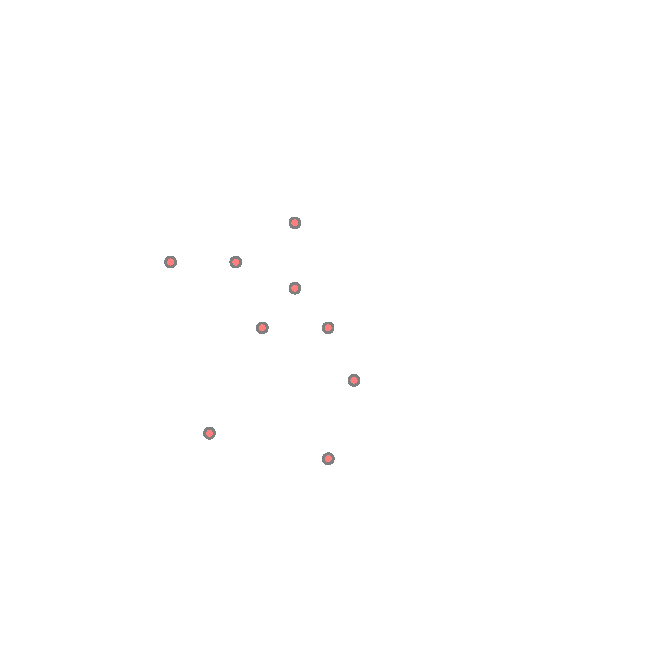
\includegraphics[height = 1.65in]{test_sample.tikz}
          \label{fig:test}}
          \subfloat[]{\includegraphics[height = 1.65in]{plsim_153.tikz}
          \label{fig:sim_lo}}
          \subfloat[]{\includegraphics[height = 1.65in]{plsim_75.tikz}
          \label{fig:sim_hi}}
          \caption{(a) Sample distribution. Simulation of the reconstructed sample image at: (b) $\Re k_{\p} = 39.5$ (c) $\Re k_{\p} = 80$}
          \label{fig:simulation}
        \end{figure}
      \end{frame}
      %             % ------------------------------------------------------------
      %             % ------------------------------------------------------------
      %             % ------------------------------------------------------------
      %             % ------------------------------------------------------------
      %             % ------------------------------------------------------------
      %             % ------------------------------------------------------------
      %             % ------------------------------------------------------------
      %             % ------------------------------------------------------------
      %             % ------------------------------------------------------------
      %             % ------------------------------------------------------------
      %             % ------------------------------------------------------------
      %             % ------------------------------------------------------------
      %             % ------------------------------------------------------------
      %             % ------------------------------------------------------------
      %             % ------------------------------------------------------------
      %             % ------------------------------------------------------------
      %             % ------------------------------------------------------------
      %             % ------------------------------------------------------------
      %             % ------------------------------------------------------------
      %             % ------------------------------------------------------------
      %             % ------------------------------------------------------------
                  \section{Conclusion}
                  \begin{frame}
                    \frametitle{Summary}
                    \framesubtitle{Two-dimensional plasmonic devices}
                    \begin{itemize}
                      \item Subwavelength wave phenomena at optical and terahertz frequencies
                      \item Realization of terahertz sources and sensors
                      \item 2D nature of waves permits subwavelength confinement
                      \item Plasmonic activity
                      \item Nanoscale imaging using terahertz plasma waves
                    \end{itemize}
                  \end{frame}
      %             % ------------------------------------------------------------
      %             % ------------------------------------------------------------
      %             % ------------------------------------------------------------
      %             % ------------------------------------------------------------
      %             % ------------------------------------------------------------
      %             % ------------------------------------------------------------
      %             % ------------------------------------------------------------
                  \begin{frame}
                    \frametitle{Acknowledgements}
                    \framesubtitle{Sponsorship}
                    \begin{itemize}
                      \item The Fulbright Program
                    \end{itemize}
                    \begin{figure}
                      \centering
                      \def\svgwidth{.4\linewidth}
                      \input{figures/fulbright.pdf_tex}
                      % \caption{(a). Actual and its equivalent models for the (b) external and, (c) Internal region }
                    \end{figure}
                  \end{frame}
      %             % ------------------------------------------------------------
      %             % ------------------------------------------------------------
      %             % ------------------------------------------------------------
      %             % ------------------------------------------------------------
      %             % ------------------------------------------------------------
      %             % ------------------------------------------------------------
      %             % ------------------------------------------------------------
                  \begin{frame}[plain,c]
                    \begin{center}
                      \Huge Thank you!
                    \end{center}
                  \end{frame}
      %             % ------------------------------------------------------------
      %             % ------------------------------------------------------------
      %             % ------------------------------------------------------------
      %             % ------------------------------------------------------------
      %             % ------------------------------------------------------------
      %             % ------------------------------------------------------------
      %             % ------------------------------------------------------------
                  \begin{frame}[plain,c]
                    \begin{center}
                      \Huge Questions?
                    \end{center}
                  \end{frame}
                  \end{document}
